\documentclass{article}
\usepackage[x11names]{xcolor}
\usepackage{amsmath}
\usepackage{graphicx}
\usepackage{amssymb}
\begin{document}
\textbf{fatgraph name: L}
\definecolor{c0}{rgb}{0.5529411764705883, 0.8274509803921568, 0.7803921568627451}
\definecolor{c1}{rgb}{1.0, 1.0, 0.7019607843137254}
\definecolor{c2}{rgb}{0.7450980392156863, 0.7294117647058823, 0.8549019607843137}
\definecolor{c3}{rgb}{0.984313725490196, 0.5019607843137255, 0.4470588235294118}
\definecolor{c4}{rgb}{0.5019607843137255, 0.6941176470588235, 0.8274509803921568}
\definecolor{c5}{rgb}{0.9921568627450981, 0.7058823529411765, 0.3843137254901961}
\definecolor{c6}{rgb}{0.7019607843137254, 0.8705882352941177, 0.4117647058823529}
\definecolor{c7}{rgb}{0.9882352941176471, 0.803921568627451, 0.8980392156862745}
\definecolor{c8}{rgb}{0.8509803921568627, 0.8509803921568627, 0.8509803921568627}
\definecolor{c9}{rgb}{0.7372549019607844, 0.5019607843137255, 0.7411764705882353}
\definecolor{c10}{rgb}{0.8, 0.9215686274509803, 0.7725490196078432}
\definecolor{c11}{rgb}{1.0, 0.9294117647058824, 0.43529411764705883}
\begin{center}
\begin{figure}[h]
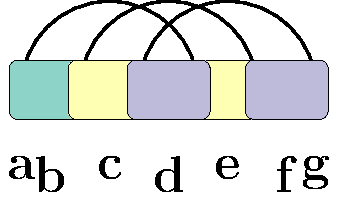
\includegraphics[width=\textwidth]{results/colored_dbn/colored_dbn_L.pdf}
\end{figure}
\end{center}
first and last anchors, already given: $ a , g $
$$ A =\min_{ b,c,d,e,f } \left( \colorbox{c2}{$C_{\boxtimes}$}[a,b,d,e]+B[f,d,c,a]+\colorbox{c1}{$C_{\boxtimes}$}[b,c,e,f]\right) $$
$$ B\left[ a,c,d,f \right] =\min_{  } \left( \colorbox{c0}{$C_{\boxtimes}$}[c,d,f,g]\right) $$
\end{document}
